\chapter{Contribution}
\label{ch:contrib}

This chapter presents what was built and why. The artefact produced is an LQN solver named \texttt{SolverLNSimple}. The established comparators (LINE's \texttt{SolverLN} \cite{casale2024} and LQNS V5 \cite{franks2009,franks2022manual}) are mature, general-purpose solvers that have become bloated with machinery over time to handle every possible case, including interlock corrections, an \texttt{iter\_min} floor and moving-average convergence. \texttt{SolverLNSimple} is built the other way around. Each piece of machinery added responds directly to a specific case of model that the previous design could not handle. The result, though not as general-purpose as the existing solvers, is focused and efficient. The result is a solver that, on the closed-LQN models in our evaluation corpus, converges in fewer outer iterations than either comparator, and does so in less clock time, providing evidence that some iteration cost of the existing solvers is structural rather than necessary. The chapter develops six key features, each motivated by the limitations of the solver on a set of models, beginning with a minimal LQN solver (Sections~\ref{sec:contrib-step1}--\ref{sec:DRAFT-perf-optimisation}).

\section{Coupling on the ensemble}
\label{sec:contrib-baseline}
\label{sec:contrib-step1}

The starting point is the smallest LQN solver that works at all. It takes a \texttt{LayeredNetwork}, decomposes it into an ensemble of PFQN submodels via \texttt{model.getEnsemble()} (which internally calls \texttt{SolverLN.buildLayers}), and wraps a coupling-iteration loop, \texttt{iterateCoupledMva}, around a PFQN MVA kernel, \texttt{Pfqn\_mvamsKt.pfqn\_mvams}. The ensemble building and kernel is delegated deliberately as we want to compare \textit{outer} iteration counts on like terms with \texttt{SolverLN} and LQNS. Working with a different ensemble would make comparisons less like-for-like, and re-implementing MVA would only reproduce the same numerical results. The first question this minimal solver must answer is how to couple the submodels.

\subsection{The minimal solver and its first coupling}

\texttt{SolverLN.buildLayers(model)} returns one PFQN sub-\texttt{Network} per server, where each host layer server is named \texttt{P:<processorName>} and each non-REF task layer server \texttt{T:<taskName>}, with reference tasks deliberately folded into the \texttt{Clients} delays of their callees' host layers rather than given their own layer. Each submodel is therefore a standard product-form closed network, with a Delay node for the clients and a queueing node for the server. In each sweep, the solver solves every layer with \texttt{pfqn\_mvams}, which is a multi-class MVA kernel (a single class is fed as \texttt{R = 1}, producing correct single-class results while leaving room to extend to the multi-class case later), then mutates Delay and Queue service times to propagate load between layers. We call \texttt{iterateCoupledMva(maxIters, tol)} with a per-layer throughput-delta tolerance, converging when the maximum delta falls below it.

The first coupling attempt to match nodes in submodels by name. A \texttt{nameIndexMap : Map<String, List<int[]>>}, built on construction, maps each node name to the \texttt{(layer, nodeIndex)} pairs where it appears, and two update methods, \texttt{updateThinkTimeFromUtilization} (Little's-law identity \texttt{z = pop · (1 - U) / X}) and \texttt{updateServiceTimeFromResidence} (\texttt{Q / X}), write through it. It is the natural first attempt, but naive as it does not comply with what \texttt{SolverLN.buildLayers} produces.

\subsection{Failure}

Name-based coupling collapses because \texttt{SolverLN.buildLayers} does not preserve node names. It prefixes every server with \texttt{T:} or \texttt{P:} and groups all clients of the server into a single node named \texttt{Clients}. Solving with the naive solver would result in \texttt{nameIndexMap} matching only on \texttt{Clients}, \texttt{updateThinkTimeFromUtilization} zeroing the Delay think times because \texttt{Clients} IS-station utilisation $\approx$ 1 drives \texttt{z = N · (1 - U) / X} to zero, and \texttt{updateServiceTimeFromResidence} would then collapse every demand to \texttt{Exp.fitMean(0)}. The coupling channel has to be rebuilt around what \texttt{buildLayers} actually shares.

\subsection{Response}

We therefore discard name matching and re-couple submodels through the \texttt{T:} / \texttt{P:} queue-name prefixes from \texttt{SolverLN.buildLayers}. Coupling is driven instead by \texttt{queueNameToLayer} and the \texttt{MvaUtils} helpers. Similarly to the naive solver, the \texttt{Z\_callee\_host = (N - Q\_server)/X} formula updates a host layer's Clients think time and the \texttt{R\_task = Q / X} formula sets a task layer's service time.

\subsubsection*{The prefix abstraction}

Four fields are introduced at the constructor that make the prefix convention usable. \texttt{baseClientsThink : double[N\_LAYERS]} captures the initial Clients think time per layer before any coupling, \texttt{queueNameToLayer : Map<String, Integer>} maps each task / processor queue name to the index of the ensemble layer that contains it to enable layer lookup in the coupling, and auxiliary maps \texttt{taskToProcessor} and \texttt{processorToTasks} are derived from the LQN model directly to traverse the host/task relationship without having to re-walk the call graph. For modularity, we move all per-layer MVA matrix construction to a new class \texttt{MvaUtils}.

\subsubsection*{The \texttt{Z\_callee\_host} formula}

When \texttt{SolverLNSimple} solves task \texttt{T}'s layer, the host layer the processor \texttt{T} runs on needs its Clients think updated to reflect the time \texttt{T} spends away from the host server. By Little's law on a closed M/M/c sub-network, we get \texttt{Z\_callee\_host = (N - Q\_server) / X}, a formula derived from \texttt{njobs · |1 - util| / tput - thinktime}. We also find that \texttt{pfqn\_mvald}, called from \texttt{pfqn\_mvams}, returns \texttt{U = 1 - P(idle)}, representing its busy probability rather than per-server utilisation. We therefore correct this by computing \texttt{u\_per\_server = X · D / c} directly.

% TODO: check
% \emph{Worked example.} Task \texttt{T1} (single-threaded, host demand $D=0.5$), on processor \texttt{P1} (single-core), appears as the \emph{server} of its own task layer \texttt{T:T1} and as the \emph{client} of the host layer \texttt{P:P1}. Solving \texttt{T:T1} (single-server closed model, $N=3$ caller jobs, \texttt{Clients} think $Z=1$) by exact MVA, $R(n)=D\,(1+Q(n{-}1))$, $X(n)=n/(Z+R(n))$, $Q(n)=X(n)\,R(n)$, gives:

% \begin{center}
% \begin{tabular}{cccc} 
% \hline
% $n$ & $R(n)$ & $X(n)$ & $Q(n)$ \\
% \hline
% 1 & $0.500$ & $0.667$ & $0.333$ \\
% 2 & $0.667$ & $1.200$ & $0.800$ \\
% 3 & $0.900$ & $1.579$ & $1.421$ \\
% \hline
% \end{tabular}
% \end{center}

% The residence $R_{\text{task}}=Q/X=0.90$ flows \emph{upward}, becoming the service \texttt{T1}'s caller layer sees. The host think $Z_{\text{callee\_host}}=(N-Q)/X=(3-1.421)/1.579=1.00$ flows \emph{downward} into \texttt{P:P1}'s \texttt{Clients} delay. We can also compute the host utilisation $u=XD/c=0.79$.

\subsection{Rejected alternatives}

An initial ambitious approach was a complete chain-walking implementation that attempted entire solution rather than building only what solves an extremely basic LQN model, falling into exactly what we said this project should not do. The attempt consisted of parsing the LQN model directly, building task layers from the call graph, and running three MVA cases inline (IS for \texttt{c $\geq$ N}, exact FCFS for \texttt{c = 1}, Bard-Schweitzer for \texttt{c > 1}). This approach failed to account for processor contention as we only considered task layers, plus many other factors, which proved this was a much more complex solution than what we required at this stage, diverging from the motivation of the project. 

\subsection{What ensemble coupling provides}

Ensemble coupling was tested on two-layer and three-layer chain models. Whilst it is not bug-free, it finds correct results for some simple given cases, and allows us to explore further. Graph-derived coupling (Section~\ref{sec:contrib-step2}) closes these bugs, narrowing the gap to \texttt{SolverLN} towards a competent, efficient solver.

The structural lessons are that we should look to consider how the tools given to us work rather than attempting an approach, and that we need to remain mindful of the project's scope and the specific task at hand, rather than attempting complex, wholesale fixes. The coupling channel is dictated by what \texttt{SolverLN.buildLayers} shares across layers (the \texttt{T:} / \texttt{P:} server prefixes and a single \texttt{Clients} class) and therefore must be indexed by the prefix. Delegating the modelling and MVA to the ensemble allowed us to produce the smallest possible structure that lets the coupling formulas express their additive contributions to a fixed pre-coupling baseline.



\section{Graph-derived coupling}
\label{sec:contrib-step2}

When the prefix coupling solve was fed richer LQN chains, the solver produced incorrect results. Each symptom traced to a different blind spot of the prefix abstraction: the static \texttt{baseClientsThink[callerTaskLayer]} baseline read zero when the caller layer was Immediate, the \texttt{(N - Q\_server)/X} coupling formula could divide by a throughput collapsing to zero which in turn propagates \texttt{NaN}/\texttt{Infinity} through subsequent Clients writes, and \texttt{getRootRefThinkTime} would walk the call chain all the way to the REF task as we had not considered any intermediate think times. 
The response was to stop deriving coupling targets from ensemble-layer indexing as this led to too many assumptions, and instead read them from the \texttt{LayeredNetwork} graph itself, via root-REF walks, caller-chain demand sums and subtree demand checks, providing a more natural approach. 

\subsection{Failure}

To first check the prefix coupling approach and investigate any blind spots, a suite of simple LQN models was constructed by hand. When a failure was observed (\texttt{SolverLNSimple}'s result deviates from \texttt{SolverLN}), we would attempt to reproduce and pin down the exact point of failure. With the suite in place, the blind spots fall into three classes, seen in Figure~\ref{fig:cs-step2-fixtures} and described below.

\textbf{Depth $\geq$3 chains with Immediate intermediate activities.} On models with intermediate tasks with Immediate activities, \texttt{baseClientsThink[callerTaskLayer]} is initially zero, while the intermediate layer has \texttt{D = 0} and zero caller think time. The callee's MVA solve therefore sees no upstream load and converges to a meaningless fixed point.

\textbf{Immediate-leaf subtrees.} For a model where every task in some sub-tree has \texttt{getHostDemandMean() $\approx$ 0}, the \texttt{(N - Q\_server)/X} formula divides by an \texttt{X} that is essentially zero, producing \texttt{Infinity}/\texttt{NaN}s that propagate through the next sweep's Clients-think writes.

\textbf{Intermediate tasks with non-zero think times.} On models where intermediate tasks have their own think time, any REF-walking lookup, such as \texttt{getRootRefThinkTime()}, terminates at the root REF, ignoring intermediate think times along the chain.

\begin{figure}[!htbp]\centering
\tikzset{
  lqntask/.style={rectangle, rounded corners=2pt, draw=black!70, text width=11mm, align=center, minimum height=6mm, fill=blue!4},
  lqnref/.style={lqntask, fill=green!8},
  lqnimm/.style={lqntask, fill=black!12},
  lqnproc/.style={ellipse, draw=black!70, minimum width=12mm, minimum height=6mm, fill=orange!8},
  lqnca/.style={->, draw=black!70}, lqnha/.style={-, draw=black!60, dashed},
  lqnel/.style={font=\scriptsize, color=black!70}}
\begin{subfigure}[t]{0.31\textwidth}\centering
\begin{tikzpicture}[>={Stealth[length=2mm]}, font=\footnotesize]
  \node[lqnref] (r) at (0,0) {T1\\(REF)};
  \node[lqnimm, below=7mm of r] (m) {Mid\\(Imm)};
  \node[lqntask, below=7mm of m] (l) {Leaf};
  \node[lqnproc, below=7mm of l] (p) {P1};
  \draw[lqnca] (r)--(m); \draw[lqnca] (m)--(l); \draw[lqnha] (l)--(p);
\end{tikzpicture}
\caption{Depth-3 chain with Immediate intermediate demand.}
\end{subfigure}\hfill
\begin{subfigure}[t]{0.34\textwidth}\centering
\begin{tikzpicture}[>={Stealth[length=2mm]}, font=\footnotesize]
  \node[lqnref] (r) at (0,0) {T1\\(REF)};
  \node[lqnimm, below=7mm of r] (m) {Mid\\$D{\approx}0$};
  \node[lqnimm, below left=7mm and 3mm of m] (l1) {Leaf1\\$D{\approx}0$};
  \node[lqnimm, below right=7mm and 3mm of m] (l2) {Leaf2\\$D{\approx}0$};
  \draw[lqnca] (r)--(m); \draw[lqnca] (m)--(l1); \draw[lqnca] (m)--(l2);
\end{tikzpicture}
\caption{Immediate-leaf subtree.}
\end{subfigure}\hfill
\begin{subfigure}[t]{0.31\textwidth}\centering
\begin{tikzpicture}[>={Stealth[length=2mm]}, font=\footnotesize]
  \node[lqnref] (r) at (0,0) {T1\\(REF)};
  \node[lqntask, below=7mm of r] (m) {Mid\\$Z{=}z$};
  \node[lqntask, below=7mm of m] (l) {Leaf};
  \node[lqnproc, below=7mm of l] (p) {P1};
  \draw[lqnca] (r)--(m); \draw[lqnca] (m)--(l); \draw[lqnha] (l)--(p);
\end{tikzpicture}
\caption{Intermediate node with think time.}
\end{subfigure}
\caption{The three blind spots motivating graph-derived coupling.}
\label{fig:cs-step2-fixtures}
\end{figure}

The primary observation is that the prefix coupling creates an abstraction of the real information that lives in the LQN graph based on false assumptions. If we access this directly, we can gain a deeper and correct understanding of the system's behaviour, with no loss of information.


\subsection{Response}

The updated design replaces \texttt{baseClientsThink[callerTaskLayer]} indexing with a structured set of helpers that take task names as inputs and read the \texttt{LayeredNetwork} graph directly.

\subsubsection*{Chain-walk root-REF lookup}

The first chain-walking helper is \texttt{findRootThink(int startLayer)}. The previous design read the immediate caller's think directly as \texttt{baseClientsThink[callerTaskLayer]}, a single index one hop up. This is only valid in depth 2 fixtures, when the immediate caller is the root REF, but fails when an Immediate intermediate sits between the REF and the callee, returning 0 and causing the callee to see no upstream load. \texttt{findRootThink} therefore replaces this with a walk up the chain until a \texttt{R:} REF task layer is reached. We also implement a \texttt{[task $\rightarrow$ caller-service]} injection for caller task layers, the caller's service demand can be overwritten and the callee response reaches the caller's MVA solve. We also ensure \texttt{taskResidT} is reported zero for Immediate non-REF tasks, ensuring the propagated callee response is not reported as the intermediate's own service. These changes solve the depth$\geq$3 with Immediate intermediates category, but the more important headline is the shift from a single-index lookup to walking the \texttt{LayeredNetwork} graph itself.

\subsubsection*{Multi-call support}

Previously, we assumed each activity can only make one call for simplicity, however it is possible for a single activity to invoke multiple calls to its target each visit. The change adds a recursive \texttt{resolveTaskResponseTime} helper that reconstructs task response time through the call chain, multiplying through by the number of calls, \texttt{callMean}, at each step. We can then use \texttt{propagatedTaskResp = R\_task\_total $\times$ syncCallMean} in the caller-side coupling.

\subsubsection*{Structural updates above the throughput guard}

We then look to close the \texttt{Infinity}/\texttt{NaN}-propagation failure. We do so with \texttt{hasServerDemandInSubtree(calleeTask)}, another recursive callee walk, that gates \texttt{Z\_callee\_host} such that if the subtree has no server demand, we use \texttt{calleeThinkTime} directly, instead of the \texttt{max(calleeThinkTime, (N - Q\_server)/X)} form. Our approach is to make sure that clients think updates take place even when we get non-finite solutions so we can exit the degenerate state, providing a simple and structural guarantee.

\subsubsection*{Intermediate-think coupling}

To handle the case of an intermediate task with a think time, we must use the formula \texttt{Z\_callee\_clients = max(refChainThink, directCallerThink)}, where \texttt{refChainThink} sums root think time and caller demand, while \texttt{directCallerThink} sums caller task think time and its local demand. This recognises that the callee's Clients think time must equal the bottleneck's think time, considering both the REF chain and the intermediate. A similar formula handles intermediate callees for host updates: \texttt{Z\_callee\_host = max(calleeThinkTime, callerChainZ) + (R\_task\_total − calleeLocalDemand)}, where the subtraction avoids double-counting because the host server already provides \texttt{calleeLocalDemand}.

\subsection{Rejected alternatives}

Several fixes were attempted before consolidating on the final graph-derived design, all ending up superseded or at a dead-end. Index based fixes such as layer index in \texttt{baseClientsThink[callerTaskLayer] $\rightarrow$ baseClientsThink[l]}, per-layer-N overrides in \texttt{MvaUtils.buildN} and \texttt{taskCalledByTask} reverse maps were attempted, trying local fixes. Propagation-based fixes were also looked at, including two-phase Jacobi / elevator sweeps, \texttt{pendingUpdates} deferred-coupling buffering and a \texttt{pendingCalleeUpdates}-array implementation, exploring if the current coupling behaviour was truly sound. The significance of these rejected experiments is that many local fixes to the prefix design were tried before recognising that the abstraction itself had to be replaced.

\subsection{What graph-derived coupling provides}

Graph-derived coupling enables the handling of depth$\geq$3 chains with Immediate intermediate activities, Immediate-leaf subtrees without \texttt{NaN} propagation, intermediate tasks with their own think times and single-class chains of arbitrary depth. The coupling derivation has now moved from the name matching baseline, to prefix indexing, and now to graph traversal (functions in \texttt{LqnGraph} helper), emerged from the problem at hand and became the foundation for the rest of the solver. We also learn the value of structural fixes over local ones, creating a robust solution that can handle failures and allows the solver to be extended easily.

 



\section{Multi-class support}
\label{sec:contrib-step3}

When the single-class machinery so far developed met a multi-class LQN topology, where multiple reference tasks can call shared tasks, it could not represent the per-caller demands in any single class, aggregating instead. The response was to handle each class directly. We feed multi-class demands per layer into \texttt{pfqn\_mvams}, cap per-\texttt{T:}-layer populations to the minimum effective \texttt{N}, split \texttt{callMean} into its two semantically distinct uses, and mutate the ensemble's host-layer class topology to recover the per-caller information.

\subsection{Failure}

Our first action is once again to create groups of models, this time specifically multi-class ones, that fail. We determine Category A (multiple REF tasks that call their own submodels, inducing no sharing), Category B (multiple REF tasks calling a shared server with the same demand) and Category C (multiple REF tasks calling a shared m-server with asymmetric demands) as the three categories that will enable us to diagnose the system, shown in Figure~\ref{fig:cs-step3-categories}.

\begin{figure}[!htbp]\centering
\tikzset{
  lqntask/.style={rectangle, rounded corners=2pt, draw=black!70, text width=11mm, align=center, minimum height=6mm, fill=blue!4},
  lqnref/.style={lqntask, fill=green!8},
  lqnproc/.style={ellipse, draw=black!70, minimum width=12mm, minimum height=6mm, fill=orange!8},
  lqnca/.style={->, draw=black!70}, lqnha/.style={-, draw=black!60, dashed},
  lqnel/.style={font=\scriptsize, color=black!70}}
\begin{subfigure}[t]{0.31\textwidth}\centering
\begin{tikzpicture}[>={Stealth[length=2mm]}, font=\footnotesize]
  \node[lqnref] (r1) at (0,0) {T1};
  \node[lqnref] (r2) at (1.8,0) {T2};
  \node[lqntask, below=7mm of r1] (s1) {S1};
  \node[lqntask, below=7mm of r2] (s2) {S2};
  \node[lqnproc, below=7mm of s1] (p1) {P1};
  \node[lqnproc, below=7mm of s2] (p2) {P2};
  \draw[lqnca] (r1)--(s1); \draw[lqnca] (r2)--(s2);
  \draw[lqnha] (s1)--(p1); \draw[lqnha] (s2)--(p2);
\end{tikzpicture}
\caption{Category A: independent submodels (no sharing).}
\end{subfigure}\hfill
\begin{subfigure}[t]{0.31\textwidth}\centering
\begin{tikzpicture}[>={Stealth[length=2mm]}, font=\footnotesize]
  \node[lqnref] (r1) at (0,0) {T1};
  \node[lqnref] (r2) at (1.8,0) {T2};
  \node[lqntask, below=8mm of $(r1)!0.5!(r2)$] (s) {Shared\\$D$ equal};
  \node[lqnproc, below=7mm of s] (p) {P};
  \draw[lqnca] (r1)--(s); \draw[lqnca] (r2)--(s); \draw[lqnha] (s)--(p);
\end{tikzpicture}
\caption{Category B: shared server, symmetric demand.}
\end{subfigure}\hfill
\begin{subfigure}[t]{0.31\textwidth}\centering
\begin{tikzpicture}[>={Stealth[length=2mm]}, font=\footnotesize]
  \node[lqnref] (r1) at (0,0) {T1};
  \node[lqnref] (r2) at (1.8,0) {T2};
  \node[lqntask, below=8mm of $(r1)!0.5!(r2)$] (s) {Shared\\($m$-srv)};
  \node[lqnproc, below=7mm of s] (p) {P ($c$)};
  \draw[lqnca] (r1)-- node[lqnel,left]{$D_a$} (s);
  \draw[lqnca] (r2)-- node[lqnel,right]{$D_b$} (s);
  \draw[lqnha] (s)--(p);
\end{tikzpicture}
\caption{Category C: shared $m$-server, \emph{asymmetric} demand ($D_a\neq D_b$).}
\end{subfigure}
\caption{The multi-class fixture categories.}
\label{fig:cs-step3-categories}
\end{figure}

These fixtures expose two key blind spots. We use \textit{single-class matrix builders} to call MVA with, following our minimal solution paradigm where up to this point we only had one class, which is what the solver uses \texttt{MvaUtils.getMainClass} in the matrix builders. We also only consider a single aggregate class in our models, which works when we are met with multiple classes with equal demands, but falls apart as soon as we see \textit{asymmetric per-caller demands}, losing the ability to recover per-caller results.

\subsection{Response}

% TODO

\subsubsection*{Multi-class per-layer demands}

Our previous design consideration of choosing to delegate MVA to \texttt{pfqn\_mvams} allows us to feed multi-class demands into the MVA naturally, as it already supports \texttt{R > 1} (M $\times$ R demand, 1 $\times$ R population, 1 $\times$ R think-time).

We obtain the multi-class demands by iterating the ensemble layers and feeding the server demands into the MVA matrix builders. For each layer we identify \texttt{tasksOnServer} (the single task for a \texttt{T:} layer, every task on the processor for a \texttt{P:} server), assigning a service demand to each closed class via one of two rules. An aggregate \texttt{T:xxx} class on a \texttt{P:} server represents the hosted task, where its demand is the caller-multiplicity-weighted mean host demand. For per-caller \texttt{R:caller} classes, we sum \texttt{callMean $\times$ serverAct.getHostDemandMean()} over sync calls to server entries.

\texttt{MvaUtils} extends to multi-class by introducing \texttt{getClosedClasses} to return all closed classes with \texttt{N > 0} and modifying \texttt{buildDemandMatrix} to return M $\times$ R, and \texttt{buildN} and \texttt{buildThinkTimeMatrix} to return 1 $\times$ R. The \texttt{iterateCoupledMva} coupling loop is updated to iterate over all classes, tracking convergence via per-class-per-layer throughput, implementing per-class Clients-think writes, per-class \texttt{R\_task\_r} in the \texttt{[task $\rightarrow$ host]} loop and per-class \texttt{R\_proc\_r} in the host-submodel branch. Category A correctness (no sharing, block-diagonal demand matrices) falls out as the degenerate case of the multi-class machinery.


\subsubsection*{Multiplicity per-layer cap}

Whilst not explicitly a multi-class issue, the multi-class fixtures helped us discover an issue with the solver's population cap logic. We implement \texttt{enforceMaxMult}. It sums caller-class populations per \texttt{T:} layer into a \texttt{taskEffectiveN} map, then for each \texttt{P:} layer it finds the minimum effective \texttt{N} across its hosted \texttt{T:} classes, and caps \texttt{T:} classes whose \texttt{getNumberOfJobs()} exceeds that minimum. This ensures that bottleneck demands are properly managed, and non-bottleneck layers are not capped. We do this without touching the processor server count or the REF class directly, so no class-instance mutation can leak across layers. This is because \texttt{LayeredNetwork.getEnsemble()} shares \texttt{JobClass} instances across layers, meaning any solver that needs per-layer class semantics must either avoid mutating classes or add new classes rather than mutating existing ones.

\subsubsection*{Per-class QLen attribution}

The third sub-move addresses the residual after the first two: \texttt{taskQLen.put(taskName, q)} stores only class-0 QLen, so all activity queue lengths are wrongly reported as the class-0 QLen. The deeper structural diagnosis is that "callMean" was being asked to do two conflicting jobs (Throughput scaling requires the \textit{max} per caller to convert a leaf task's per-visit throughput into its per-call rate, and \textit{QLen apportionment} needs the \textit{sum} across callers to fairly split the shared queue's length across callers). A single overloaded function cannot serve both sites.

To implement this fix, we first split \texttt{getTotalInboundCallMean} into \texttt{getTotalInboundCallMean} and \texttt{getSumInboundCallMean}, plus \texttt{getCallerTotalCallMean(callerTask, targetTask)} for per-caller-pair lookups. Secondly, a parallel map \texttt{taskClassQLen : Map<String, Map<String, Double>>} tracks per-caller QLen at each task, populated from the per-class MVA \texttt{Q[serverIdx, rc]} rather than a pooled \texttt{taskQLen[taskName]}. Finally, \texttt{applyRefTaskInheritance}'s signature is extended to take \texttt{taskClassQLen}, and the \texttt{q\_callee} apportionment becomes \texttt{q\_callee += (m / callerTotalCM) $\times$ classSpecificQ} when class-specific QLen is available, replacing the naive \texttt{q\_callee += classSpecificQ}.

\subsubsection*{Mutating the ensemble's class topology}

The fourth sub-move mutates the ensemble's class topology rather than refining coupling formulas that operate on it. The trigger is Category C (asymmetric per-caller demands), diagnosing that no coupling formula can recover the per-caller information from a single aggregate class. We first attempted a mini PFQN solver that ran in-place on the ensemble at every iteration, calculating the necessary values. Although this produced the correct results, it required a lot of special-case machinery and side-channel computation, which is why we opted to represent the per-caller demands as new classes directly in the ensemble, adding per-caller \texttt{R:} classes to the ensemble at construction, disabling the aggregate. 

The new method walks each \texttt{P:} host layer, where the hosted task is INF-scheduled, called by multiple REF tasks and does not make sync calls itself. For each such layer it adds new \texttt{ClosedClass("R:" + callerName, mult, clientDelay)} instances marked \texttt{setReferenceClass(true)}, disables the aggregate class via \texttt{setPopulation(0)} and \texttt{Disabled.getInstance()} on both Clients and server queues, assigns per-class \texttt{Exp.fitMean(callerThink)} at Clients and \texttt{Exp.fitMean(callerDemand)} at the server, and rebuilds the routing matrix \texttt{Clients ↔ Queue} for every class.

\texttt{perCallerHostDemand : Map<String, Map<String, Double>>} and \texttt{aggregateHostDemand : Map<String, Double>} capture the demands collected during the constructor's per-class block. The \texttt{iterateCoupledMva} loop adds an early branch that feeds per-class \texttt{R\_proc\_r} directly into the hosted task's server and skips the \texttt{Z\_callee\_host} update for rebuilt layers. The result extraction has to be extended too, adding a per-rebuilt-layer aggregation branch summing \texttt{q\_r} / \texttt{x\_r} over per-caller classes back to the hosted task.

This is the only capability that mutates ensemble structure directly, rather than complicating the coupling formulas.

\subsection{Rejected alternatives}

We attempted many alternatives to the final design, each rejected for a different reason. Multi-class support is where the ensemble's class topology first proved misaligned with the LQN's class structure, forcing us to mutate it to recover the necessary information. The rejected alternatives include:

We considered \texttt{solveIndependentChains} as a Category A initial solution and performance optimisation, however decided against this as it was not necessary since we can solve multi-class models natively with \texttt{pfqn\_mvams}. Instead, this would add extra code paths, bloating the solution and going against the spirit of this project.

Two fixes we attempted were using the LQN struct's \texttt{maxmult} array to cap populations directly, and walking the caller chain to compute an effective multiplicity. Both hit the architectural blocker of \texttt{LayeredNetwork.getEnsemble()} returning layers sharing identical \texttt{JobClass} object instances across layers. When \texttt{setPopulation()} was called on a class, it would cause unintended cross-layer population mutations, which motivated our non-mutating \texttt{enforceMaxMult} approach.

Each alternative approach was implemented enough to produce numerical results before being reverted. After rejecting the mini PFQN approach, we first looked at a per-class scaling factor \texttt{D\_r / D\_agg} at the coupling site. We then looked at modifying \texttt{MvaUtils.callMVA} to dispatch to \texttt{pfqn\_bs} when all non-Delay rows have a single server. Finally, we replaced the rebuilt-layer skip-guard with a per-class dynamic Z update in the FCFS coupling branch. However, numerical errors remained in each of these approaches, which is why we chose the more ambitious structural mutation of the ensemble's class topology. 

\subsection{What multi-class support provides}

Multi-class support handles multi-class LQNs within a 4.9\% tolerance. This residual is attributable to \texttt{SolverLN}'s \texttt{N=0} structural classes plus class-switching routing, which our simple solver deliberately does not replicate for simplicity. Across its four sub-moves, multi-class support teaches distinct lessons. Firstly, adding multi-class support did not require new MVA machinery, instead just requiring richer inputs for the MVA kernel. This is a recurring pattern across the build, with the project's contribution being structure, rather than re-inventing the algorithms that LINE already gets right. Secondly, we learn that we should not always pick the first correct solution as it may not align with the goals of the project, as seen with the mini-PFQN approach. Finally, we learnt that whilst the ensemble is a powerful abstraction, it is not perfect. We must still look at ways to read the LQN graph directly, or mutate the ensemble's structure such that we can handle cases in a simpler way than \texttt{SolverLN}. The decision not to follow \texttt{SolverLN}'s approach directly is the project being honest about where its discipline matters and what "errors" are real and what are artefacts of the solver, considering the efficiency-accuracy trade-off.



%% (step-3 figure and worked example integrated into the prose above)

\section{An MVA kernel for LQN-shaped inputs}
\label{sec:contrib-step4}

When the multi-class solver was run on the topologies that arise in larger LQN ensembles, such as large population models or deep chains, the \texttt{jline.api.pfqn.ld.Pfqn\_mvald} kernel, called from \texttt{Pfqn\_mvamsKt.pfqn\_mvams}, was both quadratically slow (roughly 60 s total test runtime at \texttt{N = 200}, decomposing into approximately 2.5 s per layer solve across all sweeps and layers) and numerically wrong on IS topologies (throughput collapsed at \texttt{N = 100}). The response was three layered moves, each responding to a different flaw. These were re-implementing the LD recursion with primitive \texttt{double[]} arrays in a local \texttt{MvaLd} to prevent slow execution from matrix multiplication sparseness, an AMVA path for \texttt{prodN > exactLatticeMax = 500} in \texttt{MvaAmva} for large models, and partitioning IS stations before MVA dispatch to contribute to \texttt{Z} rather than to the lattice. This is the build's headline performance work.

\subsection{Failure}

The opening trigger is a network with \texttt{N=200} single-class multi-server model. With the current solver, each layer solve takes roughly 2.5 s, and across all iterations of all layers the full test runs in about 60s. The kernel causing the slow execution is \texttt{jline.api.pfqn.ld.Pfqn\_mvald}, the load-dependent MVA implementation. Its \texttt{pi} table (the marginal-queue-length probabilities \texttt{pi(k|n)} indexed by \texttt{(k, n)}, used in the LD recursion) is allocated as a sparse-CSC \texttt{Matrix}. The MVA recursion accesses the table densely, reading every \texttt{(k, n)} cell at step. These dense $O(N^2)$ \texttt{get}/\texttt{set} operations against a sparse-CSC matrix is the bottleneck. The second flaw is numerical and surfaces independently, where we note that instability starts at \texttt{N = 20} in the 2-station IS topology, leading to collapsed throughputs. Both flaws point to the fact that \texttt{Pfqn\_mvald} is the wrong kernel for some LQN-shaped inputs, as it is too slow for dense large-N accesses, and wrong on IS-only inputs.

\subsection{Response}

The three moves respond to the two flaws by fixing the representation, adding an approximate path, and partitioning IS stations before dispatch. Each move is intentionally narrow, leading to a clean solution.

\subsubsection*{Re-implementing LD recursion with primitive arrays}

The first move introduces \texttt{MvaLd.java} in \texttt{ln\_simple/mva/}. \texttt{MvaLd} is a faithful, numerically identical re-implementation of \texttt{jline.api.pfqn.ld.pfqn\_mvald} (same recursion, same accumulation order, same stabilisation rule), with the difference being that we are using primitive \texttt{double[]} arrays for the marginal queue-length probability tables \texttt{pi(k|n)} and per-population throughputs \texttt{Xs} instead of sparse-CSC matrices. We index the flat \texttt{double[]} array via \texttt{(k * (prodN+1)) + n}, where \texttt{prodN = Π\_r (N[r]+1)}. This allows the dense access pattern in the LD recursion runs at primitive-array speed rather than at sparse-CSC speed. \texttt{MvaInputs.callMVA} is rewritten to route the closed multi-server case through \texttt{MvaLd} instead of the call to \texttt{Pfqn\_mvamsKt.pfqn\_mvams}, as this was when it was routed to \texttt{pfqn\_mvald}. Single-server topologies therefore still use the existing kernel for simplicity.



\subsubsection*{AMVA dispatch for large \texttt{prodN}}

\texttt{MvaLd}'s \texttt{O(prodN · Nsum)} lattice enumeration is still expensive at very large \texttt{N}. The next move adds an approximate MVA path, known to be a more efficient solution to traditional MVA whilst still providing accurate results for sufficient \texttt{N}. We perform a threshold sweep over 12 models $\times$ 6 thresholds as a rigorous evaluation for when we should dispatch to AMVA. Six concrete alternatives were evaluated and rejected before settling: three candidate kernels (Naive Schweitzer, Krzesinski Linearizer, plain Bard-Schweitzer) and two global policies (all-LD, all-AMVA) were rejected in favour of the \texttt{prodN $\leq$ 500} threshold.

\textit{Naive Schweitzer multi-server BS} (\texttt{W = L · (1 + Q · (N − 1) / (N · c))}) resulted in a 17--50\% error versus \texttt{SolverLN}, making it too inaccurate to be a candidate. \textit{Krzesinski Linearizer (\texttt{pfqn\_linearizermsKt})} (\texttt{PB = 2·sumQ/(pop+1-nservers)}) goes negative when \texttt{nservers $\approx$ ntot}, which the project's specific input shape of INF-folded inputs forced. \textit{Plain Bard-Schweitzer (\texttt{pfqn\_bsKt})} returned per-server \texttt{Q} not total, meaning the patch would need a wrapper, so we abandoned in favour of an in-place implementation.

Understanding \texttt{SolverLN}'s own multi-server AMVA path (\texttt{jline/solvers/mva/handlers/Solver\_amva.kt}), we gathered that it uses the Seidmann/Rolia transform explicitly. It applies \texttt{L' = L/c} and \texttt{Z' = Z + $\Sigma$ L·(c-1)/c}, then plain BS. We therefore implement the \texttt{MvaAmva} class with the same logic, once again in primitive \texttt{double[]} form. The transformation gives us \texttt{L'[i,r] = L[i,r] / c[i]} \texttt{ΔZ[r] = Σ\_q L[q,r] · (c[q] − 1) / c[q]}. We then use Bard-Schweitzer iteration on the transformed inputs \texttt{(L', Z + ΔZ)}, followed by reconstruction of the total queue length \texttt{Q\_total[i,r] = Q\_BS[q,r] + X[r] · L[i,r] · (c[i] − 1) / c[i]}. The project's discipline, match \texttt{SolverLN}'s idiom where it is right and depart where it has reason to, is once again on display.



\subsubsection*{Partition IS stations before dispatch}

After resolving the performance issues, the final move addresses the numerical flaw we have been ignoring.

Our initial solution was to not create \texttt{T:} layers for INF-scheduled tasks at all, restructuring how the ensemble feeds into the solver. As they contribute no service demand, we are able to do this, propagating their effects via the per-caller host-layer mechanism. Whilst this solution matches mature solvers such as LQNS, it required a large restructuring of the solver, so we looked for a localised fix.

Once again, we looked at what \texttt{SolverLN} does. \texttt{SolverLN} partitions stations by \texttt{SchedStrategy} before passing them to MVA, such that INF servers contribute their service demand to the effective \texttt{Z} and are reconstructed post-MVA, so that the MVA recursion never sees them. We rewrite \texttt{MvaInputs.callMVA} to do just that. For each station with \texttt{S[i] >= ntot} (effectively IS), we mark \texttt{isInf[i] = true}, fold \texttt{L[i,r]} into \texttt{zEff[r]} and zero \texttt{lEff[i,r]}. If every station is IS, we can short-circuit via \texttt{analyticalISResult}: \texttt{X[r] = N[r] / Z\_eff[r]}, \texttt{Q[i,r] = X[r] · L\_original[i,r]}, \texttt{U[i] = 0}. Otherwise, we dispatch to \texttt{MvaAmva} or \texttt{MvaLd} on the non-IS subset only, patching the IS rows of \texttt{Q} back in via \texttt{rebuildInfStationQ} post-MVA.

\subsection{What the MVA kernel provides}

The quantitative result from this work is huge. Our \texttt{N=200} model drops from approximately 60 s per test run to just 0.1 s, a 600$\times$ speedup, from re-implementing \texttt{Pfqn\_mvald}'s recursion with primitive arrays. The AMVA dispatch gives us a further speedup for large models, and the IS partitioning fixes a numerical issue. Figure~\ref{fig:cs-step4-mva} plots all three effects: the primitive-array \texttt{MvaLd} and \texttt{MvaAmva} kernels against their sparse-\texttt{Matrix} equivalents, and the \texttt{prodN}=500 dispatch threshold between them.
 
One lesson we learnt was that sometimes the LINE abstractions we use actually hide representational costs. Despite sparse-CSC being a sensible library default, it was the wrong choice on a workload it was not designed for. Another lesson was that it can be better to evaluate heuristic thresholds empirically rather than arguing from theory, as competing error modes provide a non-monotone trade-off. Finally, when a mature reference solver implementation is available, it pays to try simpler approaches first and measure where they fail before reading the reference's source. These specific failure modes reveal which constraints the reference's design is actually solving, and what fixes need to be made, so the resulting code can provide the correct minimal solution. 
 
\begin{figure}[!htbp]\centering 
\tikzset{
  lqntask/.style={rectangle, rounded corners=2pt, draw=black!70, text width=11mm, align=center, minimum height=6mm, fill=blue!4},
  lqnref/.style={lqntask, fill=green!8},
  lqnproc/.style={ellipse, draw=black!70, minimum width=12mm, minimum height=6mm, fill=orange!8},
  lqnca/.style={->, draw=black!70}, lqnha/.style={-, draw=black!60, dashed},
  lqnel/.style={font=\scriptsize, color=black!70}}
\begin{subfigure}[t]{0.32\textwidth}\centering
\resizebox{\linewidth}{!}{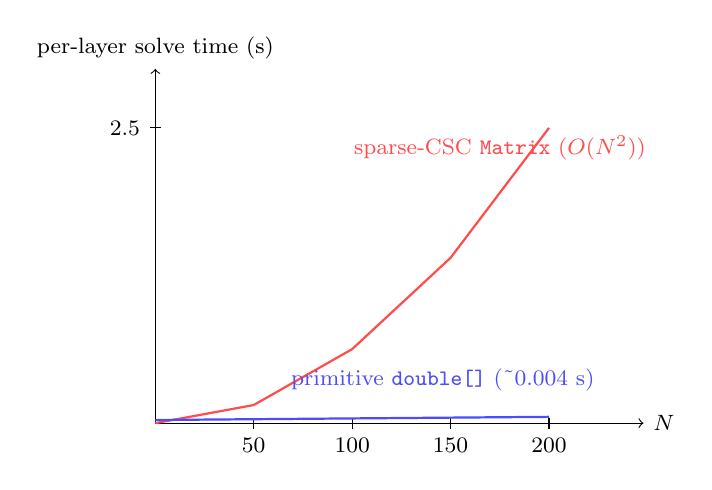
\begin{tikzpicture}[font=\footnotesize]
  \draw[->] (0,0) -- (6.2,0) node[right]{$N$};
  \draw[->] (0,0) -- (0,4.5) node[above]{per-layer solve time (s)};
  \foreach \x/\l in {1.25/50,2.5/100,3.75/150,5/200} \draw (\x,2pt)--(\x,-2pt) node[below]{\l};
  \draw (2pt,3.75)--(-2pt,3.75) node[left]{2.5};
  \draw[thick, red!70] plot coordinates {(0,0)(1.25,0.23)(2.5,0.94)(3.75,2.1)(5,3.75)};
  \node[red!70, anchor=west] at (2.4,3.5) {sparse-CSC \texttt{Matrix} ($O(N^2)$)};
  \draw[thick, blue!70] plot coordinates {(0,0.04)(1.25,0.05)(2.5,0.06)(3.75,0.07)(5,0.08)};
  \node[blue!70, anchor=west] at (1.6,0.55) {primitive \texttt{double[]} (\textasciitilde0.004 s)}; 
\end{tikzpicture}}
\caption{primitive \texttt{double[]} \texttt{MvaLd} vs. sparse-CSC \texttt{Matrix} \texttt{Pfqn\_mvald} per solve across $N$.}
\end{subfigure}\hfill 
\begin{subfigure}[t]{0.32\textwidth}\centering
\resizebox{\linewidth}{!}{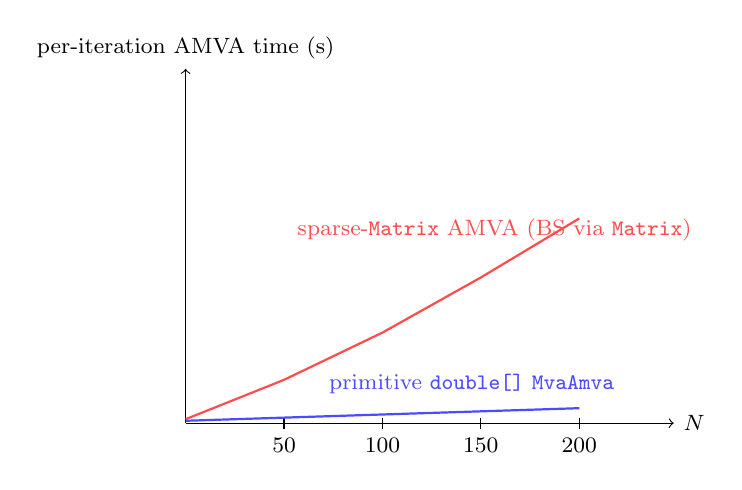
\begin{tikzpicture}[font=\footnotesize]
  \draw[->] (0,0)--(6.2,0) node[right]{$N$};
  \draw[->] (0,0)--(0,4.5) node[above]{per-iteration AMVA time (s)};
  \foreach \x/\l in {1.25/50,2.5/100,3.75/150,5/200} \draw (\x,2pt)--(\x,-2pt) node[below]{\l};
  \draw[thick,red!70] plot coordinates {(0,0.05)(1.25,0.55)(2.5,1.15)(3.75,1.85)(5,2.6)};
  \node[red!70,anchor=west] at (1.3,2.45){sparse-\texttt{Matrix} AMVA (BS via \texttt{Matrix})};
  \draw[thick,blue!70] plot coordinates {(0,0.03)(1.25,0.07)(2.5,0.11)(3.75,0.15)(5,0.19)};
  \node[blue!70,anchor=west] at (1.7,0.5){primitive \texttt{double[]} \texttt{MvaAmva}};
\end{tikzpicture}}
\caption{primitive \texttt{double[]} \texttt{MvaAmva} vs. sparse-\texttt{Matrix} AMVA per iteration across $N$.}
\end{subfigure}\hfill
\begin{subfigure}[t]{0.32\textwidth}\centering
\resizebox{\linewidth}{!}{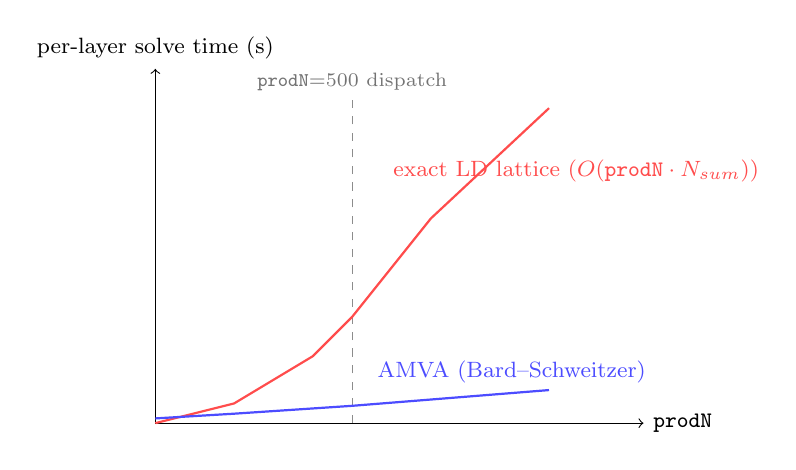
\begin{tikzpicture}[font=\footnotesize]
  \draw[->] (0,0)--(6.2,0) node[right]{$\texttt{prodN}$};
  \draw[->] (0,0)--(0,4.5) node[above]{per-layer solve time (s)};
  \draw[dashed,black!45] (2.5,0)--(2.5,4.1);
  \node[black!55,anchor=south,font=\scriptsize] at (2.5,4.1){\texttt{prodN}=500 dispatch};
  \draw[thick,red!70] plot coordinates {(0,0)(1,0.25)(2,0.85)(2.5,1.35)(3.5,2.6)(5,4.0)};
  \node[red!70,anchor=west] at (2.9,3.2){exact LD lattice ($O(\texttt{prodN}\cdot N_{\text{sum}})$)};
  \draw[thick,blue!70] plot coordinates {(0,0.06)(1,0.12)(2.5,0.22)(3.5,0.30)(5,0.42)};
  \node[blue!70,anchor=west] at (2.7,0.65){AMVA (Bard--Schweitzer)};
\end{tikzpicture}}
\caption{\texttt{MvaLd} vs.\ \texttt{MvaAmva} across lattice size $\texttt{prodN}=\prod_r(N_r{+}1)$, showing the \texttt{prodN}=500 AMVA dispatch threshold.}
\end{subfigure}
\caption{Motivation for AMVA dispatch and primitive \texttt{MvaLd}/\texttt{MvaAmva}.}
\label{fig:cs-step4-mva}
\end{figure}



%% (step-4 plots integrated into the prose above)


\section{Fan-out callers}
\label{sec:contrib-step5}
This capability responds to the remaining fixture surfaces the build had not yet exercised. The headline failure is fan-out: when the solver meets LQN topologies where a single caller makes synchronous calls to multiple distinct callees, the coupling iteration enters a two-state limit cycle, converging in 3 iterations to a fully-saturated state. The fix adds time-at-siblings into the caller's Clients think, plus a conditional under-relaxation \texttt{Z\_RELAX\_ALPHA = 0.5} gated on \texttt{LqnGraph.callerFansOut} that keeps single-callee chains un-damped. This work also calibrates the multi-class machinery (Section~\ref{sec:contrib-step3}) against fixtures that intentionally attempt to result in a high iteration count. These combine multi-class callees with multi-entry callers.

\subsection{Failure}

Up to this point, fan-out structures were not a pattern we considered. With the current solver, the model saturates as tasks get inflated \texttt{R\_proc} from host layers written to their demand via \texttt{writeHostResponseToTaskLayerServer}. The missing fix being that on a fan-out caller, the caller's effective \texttt{Clients} think time must include time spent at each sibling callee, but currently only returns \texttt{max(refChainThink, directThink)}, trapping the iteration at a false fixed point.


\subsection{Response}

The fix starts with \texttt{LqnGraph.callerFansOut(model, taskName)}, iterating the task's activities, collecting distinct callee task names, and returns true when the set has more than one element. \texttt{SolverLNSimple.computeSiblingCalleeBlocking(callerTask, excludedCallee)} then iterates the caller's activities and accumulates \texttt{callMean × R(sibling)}, reading from \texttt{taskSojournCache}. The term is used in \texttt{computeCallerClientsThink}, \texttt{propagateHostLayerCoupling}'s per-class \texttt{newZ}, and \texttt{pushRefTaskHostResponseToCalleeClients}. 
We also apply conditional under-relaxation \texttt{Z\_RELAX\_ALPHA = 0.5} in \texttt{updateTaskLayerClientsThinks} when \texttt{callerFansOut} is true, so that single-callee chains keep their un-damped fast path whilst fan-out callers get damping to limit the oscillation from multiple simultaneously-updated channels.

\subsection{Rejected alternatives}

We also had a look at a couple of alternatives for the final design, however neither was adopted. We attempted a Little's-law warm-start with bottleneck bounds. Whilst this approach saved one iteration, it was at the cost of two new formulas, gating heuristics, and warm-start machinery, so was judged as not worth the conceptual overhead. Another approach was \texttt{relax\_omega} adaptive damping. The goal was to detect oscillation via sign-change, however for fan-out workloads, the false-saturation locks in early, meaning the adaptive damping only arrives after a bad fixed point is set. A considered approach was to gate fixed-$\alpha$ damping on a predicate that identifies fan-out callers statically (\texttt{LqnGraph.callerFansOut}), so damping is on from sweep 1 for the topology that needs it. This is the C-1 novelty candidate flagged in the related-work survey.

\subsection{Refining multi-class \texorpdfstring{$\times$}{x} multi-entry interactions}

Once the fan-out fix is in, we look to finalise any remaining bugs. Those found were per-class apportionment of pushed-back demand (had been hard-coded into a single class), per-call-vs-per-visit semantics for multi-entry callers (calls dispatched by a bound activity to multiple entries should be averaged not summed across entries, as each visit goes to one entry), summing per-class throughput and queue length in coupling propagation (had been reading class-0 only), and a leaf-vs-intermediate \texttt{cMean} distinction for sojourn-time multiplication. A results-side regression also surfaced, where a single \texttt{entryQlenFraction} map was used for both QLen and Util, as Util needs host-demand-only weighting (\texttt{X $\cdot$ D / c}) while QLen needs full per-call weighting.

\subsection{What fan-out handling provides}

Large fan-out models now converge to the correct result in roughly 24 outer iterations rather than locking in a false fixed point at 3 iterations. The multi-class $\times$ multi-entry refinement clears all regressions on the test corpus.

The structural lesson from the fan-out implementation is that the iteration's dynamical structure matters, not just per-sweep math. Gating fixed-$\alpha$ damping on a structural predicate (\texttt{callerFansOut}) means damping is on from sweep 1, avoiding the otherwise required detection iterations. However, the trade-off is that the solver cannot adapt to model classes we have not yet considered.



%% (step-5 figure and fact-check integrated into the prose above)


\section{Activity-graph awareness}
\label{sec:contrib-step6}

When the solver was fed LQN models with richer activity-graph features, its bag-of-activities reading of each entry returned incorrect results. The pre-activity-graph solver treated every entry as if its bound activity was the whole entry's per-call cost and treats every task's activities as a flat unordered bag. This therefore doesn't account for the branch probabilities, loop counts, parallelism and the synchronous-wait boundary. We solve this with a per-activity visit-weight DAG walk over \texttt{ActivityPrecedence}, an AND-fork correction that replaces the branch-sum with the inclusion-exclusion $E[\max]$ of branch demands and a phase1-phase2 split that narrows the caller-perceived demand at REPLY. Figure~\ref{fig:cs-step6-dag} shows an example activity graph that exercises these features.

\begin{figure}[!htbp]\centering
\resizebox{\textwidth}{!}{%
\begin{tikzpicture}[>={Stealth[length=2mm]}, font=\footnotesize,
  act/.style={circle, draw=black!70, fill=blue!6, minimum size=8mm, inner sep=0pt},
  ctl/.style={diamond, draw=black!70, fill=orange!12, inner sep=1pt, minimum size=5mm, font=\scriptsize},
  a/.style={->, draw=black!70}, el/.style={font=\scriptsize, color=black!70}]
  \node[act] (a0) at (0,0) {A0};
  \node[ctl] (orf) at (1.6,0) {OR};
  \node[act] (a1) at (3.2,0.9) {A1};
  \node[act] (a2) at (3.2,-0.9) {A2};
  \node[ctl] (orj) at (4.8,0) {$\cup$};
  \node[ctl] (anf) at (6.1,0) {AND};
  \node[act] (b1) at (7.6,0.9) {B1};
  \node[act] (b2) at (7.6,-0.9) {B2};
  \node[ctl] (anj) at (9.1,0) {$\parallel$};
  \node[act] (lb) at (10.7,0) {L};
  \node[act] (rp) at (12.4,0) {A$_R$};
  \draw[a] (a0)--(orf);
  \draw[a] (orf)-- node[el,above left]{$p{=}0.7$} (a1);
  \draw[a] (orf)-- node[el,below left]{$p{=}0.3$} (a2);
  \draw[a] (a1)--(orj); \draw[a] (a2)--(orj);
  \draw[a] (orj)--(anf);
  \draw[a] (anf)--(b1); \draw[a] (anf)--(b2);
  \draw[a] (b1)--(anj); \draw[a] (b2)--(anj);
  \draw[a] (anj)--(lb);
  \draw[a] (lb) to[out=60,in=120,looseness=6] node[el,above]{$\times n$} (lb);
  \draw[a] (lb)--(rp);
  \draw[densely dashed, red!70] ($(rp.north)+(0,0.35)$) -- ($(rp.south)+(0,-0.35)$)
        node[el, color=red!70, below]{reply $\to$ E (phase-1 boundary)};
\end{tikzpicture}}
\caption{An example activity graph model.}
\label{fig:cs-step6-dag}
\end{figure}
 
\subsection{Failure:}

Six biases follow from the pre-activity-graph assumptions:

\begingroup
\setlength{\itemsep}{0pt}
\setlength{\parskip}{0pt}
\setlength{\parsep}{0pt}
\setlength{\topsep}{1pt}
\begin{itemize}
\item \texttt{LqnGraph.hostDemandOfBoundActivity(Entry)} reads only the bound activity's host demand, so \textbf{multi-activity entries whose sequence runs past the bound activity are under-counted}.
 
\item \texttt{LqnGraph.perVisitCallsFromCallerToTarget}, \texttt{SolverLNSimple.computeSiblingCalleeBlocking}, and \texttt{EnsembleInitialiser.demandFromActivityToTargets} sum \texttt{callMean} over \texttt{task.getActivities()} as a flat bag, meaning \textbf{OR-fork branch probabilities are dropped}.

\item The same flat-bag read ignores how many times a loop body fires, meaning \textbf{loop counts are dropped}.

\item AND-fork / AND-join is entirely absent from the pre-activity-graph design, treating the calls as independent. Therefore, \textbf{parallel branches are summed instead of joined}.

\item A \texttt{repliesTo(E)} call ends the caller's synchronous wait at the reply, but the post-reply phase-2 work is considered in the caller's per-call demand, meaning \textbf{a phase-1 REPLY inflates the caller-perceived demand}.

\item The same folding applies when the reply sits on the bound activity rather than mid-sequence, collapsing phase 1 to that single activity, meaning \textbf{a bound-activity REPLY inflates the caller-perceived demand}.
\end{itemize}
\endgroup

\subsection{Response:}

We address these issues with a DAG walk over the entry's activity graph. Firstly, we replace the bag read with a per-activity visit weight and apply it at every call-accounting site. We then add an AND-fork join-delay correction, applied to the reported metrics after the iteration rather than inside its coupling loop. Finally, we split each demand into a phase-1 and a phase-2 part, so the caller is charged only for the work up to its reply while the processor still sees the full demand.

\subsubsection*{Visit-weight DAG walk}

We replace the bag-of-activities read with a per-activity \textit{visit weight}, derived from a DAG walk over the entry's \texttt{ActivityPrecedence} chain. We compute these weights in \texttt{LqnGraph.computeActivityVisitWeights(Task)}, summing per-entry walks for multi-entry tasks, and \texttt{computeWeightsFromBound(Task, Activity)}, a fixed-point iteration that starts at the bound activity and propagates through precedences via \texttt{applyPrecedence}. 

The precedence handling is as follows: PRE\_SEQ inherits, PRE\_AND collapses by \texttt{max}, PRE\_OR sums, POST\_SEQ takes a single forward edge, POST\_AND each successor inherits the fan-in, POST\_OR each successor inherits \texttt{fanIn $\times$ prob}, and POST\_LOOP scales by loop count. 

\texttt{hostDemandOfEntry} walks the entry's DAG and sums \texttt{visitWeight $\times$ hostDemand} over reachable activities, giving the full demand the entry contributes per call. We follow the same idea for all other call-accounting sites that read activities as a bag, including \texttt{perVisitCallsFromCallerToTarget}, the multi-class per-class loop in \texttt{propagateTaskLayerCoupling}, and \texttt{OutputTableBuilder.appendActivityRows} (where the weight instead scales reported per-activity throughput).

\subsubsection*{AND-fork E[max] correction}

We then look to handle fork-join structures. We initially assumed the caller-perceived join delay was the deterministic $\max$ of branch demands, however we eventually recognised the pattern as the inclusion-exclusion identity for the expected maximum of independent exponentials \cite{franks99}. For two parallel branches with exponential demands of means $D_1,D_2$, the expected time for \emph{both} to finish is the inclusion-exclusion expected maximum $E[\max] \;=\; D_1 + D_2 - \frac{1}{1/D_1 + 1/D_2}$. This extends to the general case of $E[\max] = \sum_{\emptyset\neq S\subseteq\{1,\dots,K\}} (-1)^{|S|+1} \left(\sum_{i\in S}\frac{1}{D_i}\right)^{-1}.$ for $K$ branches.

The implementation adds \texttt{taskHasAndFork(model, taskName)} (predicate gating the correction), \texttt{findMatchingAndJoin(precs, branchStarters)} (bijective forward-reachability), \texttt{firstReachableJoinPre(start, joinPreActs, precs)} (POST\_SEQ depth-first search), \texttt{collectBranchDemand(task, branchStart, joinPreActs, weights)} (sums \texttt{weight $\times$ hostDemand} along one branch), \texttt{andForkMaxCorrection(task, weights)} (sums $(E[\max] - \sum \text{branchDemand})$ over matched fork/join pairs), and \texttt{expectedMaxOfExponentials(means)} (inclusion-exclusion over $2^{|K|}-1$ subsets). The demand functions now have to utilise this where needed, with \texttt{hostDemandOfEntry} now collapsing parallel branches via $E[\max]$ whilst \texttt{processorDemandOfEntry} reports the full SUM.

% The throughput correction is deliberately post-iteration rather than baked into the coupling loop. For each non-REF task with AND-fork on an INF processor, walk its caller chain up to the root REF (via \texttt{findRootRefForTask}), derive \texttt{cycle = N\_ref / X\_ref - (procD - callerD)}, and re-write \texttt{taskTput}, \texttt{taskQLen}, \texttt{taskResidT}, \texttt{processorUtil}, and \texttt{taskUtil} with the corrected cycle. The iteration itself continues to use the SUM so the root-REF cycle stays consistent with LN; only the reported metrics receive the $E[\max]$ correction. \texttt{computeEntryUtilFractions} and the asym-multiclass util branch switch to \texttt{callerProcessorDemandOnTask} so processor utilisation uses SUM rather than $E[\max]$, and \texttt{OutputTableBuilder} short-circuits the entry / activity throughput-fraction split to $1.0$ on single-entry tasks (Phase 4b's correction can make \texttt{taskTput > callerTput}, which the old ratio capped wrongly).


\subsubsection*{REPLY phase-1 / phase-2 split}

When an activity calls \texttt{repliesTo(E)} mid-sequence, the caller's synchronous wait ends, and subsequent activities are post-reply background work that the processor still pays for but the caller does not directly perceive. Considering these as one inflates the caller's per-call demand by the phase-2 body. We add \texttt{phase1ActivitiesFromBound(entry, bound)} (a forward DAG walk from the bound activity along POST\_SEQ-like edges that stops at any reply activity) and \texttt{hasPhase2Background(entry)} (full reachable set minus phase 1). 

The demand functions are now split again. For example, \texttt{hostDemandOfEntryImpl} is re-parametrised over \texttt{sumBranches} and \texttt{phase1Only} flags. We now have \texttt{hostDemandOfEntry} (phase-1 only $E[\max]$ join modelling the caller-perceived synchronous wait), \texttt{processorDemandOfEntry} (full DAG sum modelling processor occupancy), \texttt{andForkCollapsedDemandOfEntry} (full DAG $E[\max]$ join isolating the AND-fork delta from the phase split) and \texttt{phase1SumDemandOfEntry} (phase-1 raw sum).

A fresh caller can arrive while phase-2 is still busy. \texttt{phase1AdjustedResponseTime} reports the caller-perceived response time $R = S_1 + \text{prOt} \cdot S_2$ (always paying the phase-1 residence $S_1$, plus the phase-2 residence $S_2$ when, with probability $\text{prOt}$, this case occurs). We get $\text{prOt}$ from a small continuous-time Markov chain over the server's three states (idle, phase-1, phase-2). Solving it under Poisson arrivals gives $\text{prOt} = \lambda \mu_1 / (\lambda \mu_2 + \mu_1 \mu_2 + \lambda \mu_1)$, however this assumes an unbounded arrival stream, which over-states the arrival rate near saturation. We replace $\lambda$ with an effective rate $\lambda_{\text{eff}} = \lambda / (1 + \rho)$, where $\rho = \lambda D / c$ is the host utilisation.

\subsection{Rejected alternatives}

To keep all host layers in consistent units, an early version threaded explicit per-cycle / per-call basis tracking through three places: the writeback, the residence-time division, and the Q scaling. Despite correctness, it was removed in favour of a one-line change to the self-demand fallback in \texttt{setAggregateHostDemand}. That one line puts every host layer into per-cycle units at the source, making all the downstream tracking redundant. Separately, POST\_LOOP with no end activity was first handled by writing only \texttt{loopCount} to the post side, but the resulting fractional self-loop did not converge fast enough. We now simply scale the loop body's existing demand by \texttt{loopCount} in place, so the repeated work is folded in directly, providing better convergence and a cleaner implementation.

The interesting question was then where to apply the corrected $E[\max]$ join. Applying it inside the iteration (through \texttt{writeHostResponseToTaskLayerServer} on each sweep) failed, but keeping the iteration on a plain SUM and applying $E[\max]$ just the once after convergence did not. The reason is that $E[\max]$ is a non-additive function of the branch residence times, whereas the iteration's demand accounting is purely additive, therefore feeding the max back in each sweep makes downstream layers treat it as an ordinary summable demand, pushing estimates through nonlinearity and converging to a wrong fixed point. 

One case left out of scope for our simple solver is an AND-fork whose sibling branches run on the same finite-server host. The branches contend for the host's servers and overlap in time, so the plain $E[\max]$ join over-estimates the join delay. Modelling that overlap correctly needs CCD compensation \cite{heidelberger83}, requiring a large amount of invasive machinery for one narrow case.


\subsection{What activity-graph awareness provides}

Activity-graph awareness lets the solver express five constructs the bound-activity model could not: multi-activity entries that sequence past the bound activity, probabilistic OR-fork branching, POST\_LOOP wrapping a call-issuing body, AND-fork / AND-join with caller-perceived $E[\max]$ join delay on INF-hosted branches and mid-sequence REPLY with post-reply phase-2 background under the three-state overtake correction. The one gap left is where a finite-server PS host under AND-fork contention would need the CCD overlap compensation we chose not to build.

The whole demand calculation is derived naturally from a single DAG traversal, where \texttt{hostDemandOfEntryImpl(sumBranches, phase1Only)} produces the four quantities the iteration, the result correction, the processor-occupancy term and the displayed caller-perceived response time need. The $E[\max]$ correction came the other way round, understanding the numerical differences to the reference solvers, and then recognising them as the Heidelberger-Trivedi identity. We also learn that the fixed-point solution can be affected if we add non-linearity to the coupling loop, hence keeping some corrections to the results only.




\section{Optimising the solver}
\label{sec:DRAFT-perf-optimisation}

After reaching a point where the solver is correct on all cases of models we consider, excluding niche edge cases and complex corrections, we look to optimise the solver's performance. While \texttt{SolverLN} and LQNS must keep their convergence machinery general enough for every model they might ever be asked to solve, we know exactly the types of models \texttt{SolverLNSimple} targets. This freedom already lets it shed iteration cost and per-query cost, but we can go further by specifically optimising for the set of models we have.

This section is performance-motivated, optimising the convergence behaviour of the outer fixed-point loop and the per-sweep cost of the topological lookups the coupling performs. We look at a limit-cycle detector in the outer loop to prevent oscillations, memoisation of the invariant topological queries to avoid redundant computations and a revision of the convergence rule and damping features. We also discuss why classical sequence acceleration does not provide benefit for our solver. The de-generalisation \texttt{SolverLNSimple} utilises, because it only ever mutates the per-class Z/D values and not the topology those queries read, means its benefit is reduced allocation rather than measurable wall-clock. A warm-start of the coupling estimates was implemented, measured, and dropped, whilst an experiment on sweep order was also tried, and despite showing minimal performance improvements we switch to a pure elevator approach that allows comparison of iterations in the Evaluation chapter to be more like-for-like. The result is a 34.7\% reduction in outer iterations across the corpus ($568 \rightarrow 371$), with a runtime decrease of 54.9\% ($1739 \text{ms} \rightarrow 784 \text{ms}$). 


\subsection{Where the cost sits}

The correct solver carries two kinds of slack, each with concrete evidence.

\textbf{Structural iteration overhead.} Despite all models expected to show correctness doing so, we found a chain + fanout model that hits the \texttt{maxIter = 100} of our outer loop. From its 14th iteration onward, the maximum throughput delta stays consistent between iterations, with state updates alternating $A \rightarrow B \rightarrow A \rightarrow B$ in a perfect two-cycle. The two-cycle is structural as our LQN coupling's feedback loop has a caller's Clients think depends on its callee's response time, which in turn depends on the caller's think. When a caller fans out into a near-saturated callee, the loop supports two locally-stable states. Another form of overhead is the convergence tolerance \texttt{$\Delta < 5e\text{-}3$}, something we haven't considered changing since its inception, being about five times tighter than the \texttt{rtol = 5e-2} the harness actually judges against, causing perhaps unnecessary tightening. Furthermore, the per-iteration update is damped at a set $\alpha = 0.5$ on both the fan-out caller think-time and the host-response write into INF tasks, halving the step toward the fixed point, on all fixtures, despite many not needing the damping.

\textbf{General-purpose query cost.} A JDK Flight Recorder (JFR) profile of the solver places \texttt{LqnGraph.findEntry} ($\sim$54 CPU samples) and \texttt{LqnGraph.findCallerTask} ($\sim$26 samples) at the top of the samples, as seen in Figure \ref{fig:DRAFT-jfr-profile}. Both are linear scans over the \texttt{LayeredNetwork} topology, called from inside the coupling stages on every sweep of every layer. The topology, however, is invariant during a solve, yet we still force the scans to recompute every sweep. That is the kind of redundancy that a stateless, model-agnostic helper must tolerate, however our specialised solver, knowing only the Z/D values change while the topology is fixed, can exploit it.

\begin{figure}[!ht]\centering
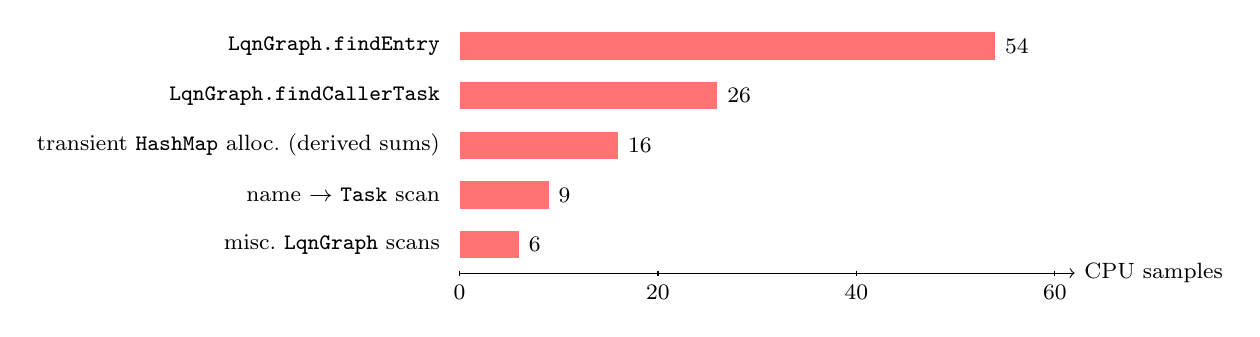
\begin{tikzpicture}[font=\footnotesize, x=1.4mm, y=7mm, scale=0.9]
  \def\barH{0.55}
  \foreach \y/\val/\name in {
      4/54/{\texttt{LqnGraph.findEntry}},
      3/26/{\texttt{LqnGraph.findCallerTask}},
      2/16/{transient \texttt{HashMap} alloc.\ (derived sums)},
      1/9/{name $\to$ \texttt{Task} scan},
      0/6/{misc.\ \texttt{LqnGraph} scans}} {
    \fill[red!55] (0,\y) rectangle (\val,\y+\barH);
    \node[anchor=west] at (\val,\y+0.5*\barH) {\val};
    \node[anchor=east] at (-1,\y+0.5*\barH) {\name};
  }
  \draw[->] (0,-0.3) -- (62,-0.3) node[right]{CPU samples};
  \foreach \x in {0,20,40,60} \draw (\x,-0.25)--(\x,-0.35) node[below]{\x};
\end{tikzpicture}
\caption{Top CPU samples in the pre-optimisation JFR profile.}
\label{fig:DRAFT-jfr-profile}
\end{figure}

\subsection{Response}

The points we make are ordered as structural features first and parameter tuning last, as whilst the features are independent of each other, the parameter choices are only safe on the state they establish, so the tuning comes once the algorithm is settled.

\subsubsection*{Limit-cycle detection}

The two-cycle is fixed not by adding damping (an $\alpha$ sweep showed the iteration count on this fixture is $\alpha$-invariant, muting the amplitude without breaking the cycle) or by extrapolating the alternating values (the classical acceleration approach that recognises non-convergence). Instead, the right response is to detect the pattern directly and exit with the answer the solver already has. 

Inside \texttt{iterateCoupledMva} we track \texttt{prevMaxDelta} and, after the existing \texttt{$\Delta <$ tol} check, test $|\Delta_k - \Delta_{k-1}| \,/\, \max(\Delta_k, \varepsilon) \;<\;$ \texttt{CYCLE\_REL} for \texttt{CYCLE\_WINDOW} consecutive iterations, gated by $\Delta_k <$ \texttt{CYCLE\_DELTA\_CAP} to keep the detector silent through the early contraction phase. The chosen constants are \texttt{WINDOW = 1}, \texttt{REL = 1e-3}, \texttt{DELTA\_CAP = 10}. This detection not only catches two-cycles where $\Delta_k = \Delta_{k-1}$, but also the smooth contraction tail of chain fixtures, where the effective contraction ratio approaches 1. The 100 iteration case now drops to 6, and chain fixtures each save a single tail iteration.

Because of these two cases, the detector returns differently depending on the shape of the stall. For a genuine two-cycle pattern, the iteration alternates across the fixed point, so their average is the better estimate. For slowly-converging chain tails, the iterations approach monotonically from one side of the fixed point, so picking the most recent result is better. We distinguish the two by checking if a sign flips between consecutive steps, $(X_k - X_{k-1})(X_{k-1} - X_{k-2}) < 0$, signifying oscillation.

\subsubsection*{Memoising the invariant topological queries}

The profiled hotspots are removed by computing each invariant query once and reusing it, and two patterns emerge. 

Single-field reads get delegated to \texttt{LayeredNetworkStruct}. For example, \texttt{findCallerTask}, the documented hotspot, is replaced by an \texttt{int[] callerOfT} in initialisation, derived from \texttt{model.getStruct().issynccaller}, instead of a triple-nested walk ($\text{Task} \rightarrow \text{Activity} \rightarrow \text{Call Destination}$) over the live LayeredNetwork object graph. A single-field lookup does better as a struct read than as a cached result, because it carries no first-call penalty and no map state.

Everything else is \emph{memoised}. A \texttt{WeakHashMap<LayeredNetwork, ModelCache>} with a volatile fast path (\texttt{lastModel}/\texttt{lastCache}), so \texttt{cacheFor()} is a pointer-identity check rather than a synchronised map lookup, holds both the name primitives (e.g. \texttt{findTask}) and the derived quantities (e.g. \texttt{computeLocalDemand}), with the same pattern applied to \texttt{MvaInputs} and to the per-submodel \texttt{Network} caches on \texttt{SolverLNSimple}. Whilst \texttt{LayeredNetworkStruct} holds similar quantities, some values may disagree with the semantics of our solver. For example, our AND-fork handling takes the max of weights whilst the struct \texttt{graph} sums branch-tip weights, so we memoise the solver's semantics directly rather than trying to re-use the struct's values.

The iteration count is unchanged as the solver runs the same algorithm and reaches the same fixed point, however each redundant topology scan that we eliminate prevents a short-lived \texttt{HashMap} from being built, saving roughly $10$--$15$k of these short-lived allocations per corpus run. Because the JVM's garbage collector has to do work in proportion to how many such objects are created and thrown away, fewer allocations means less collector work, however this was not directly measurable as the collector was never the bottleneck. What the change does surface is a profile-driven 2$\times$ performance win across the corpus ($1010 \rightarrow 497$\,ms) because the repeated name lookups were a genuine hotspot. 

\subsubsection*{Asymmetric revision of the convergence rule}

\texttt{SolverLNSimple} is primarily positioned as an \emph{efficient} solver and not a general and perfect-accuracy one, whereas \texttt{SolverLN} and LQNS are. Considering this, our original convergence and damping criteria is overspecified. 

The damping in the solver was not arbitrary, and was targeted to callers invoking more than one distinct callee, such that the new Z is under-relaxed because MVA's response slope in Z is steep near saturation, so plain fixed-point iteration alternates between saturated and unsaturated states, and that INF tasks on multi-server PS processors damp the D write since \texttt{R\_proc} fluctuates between bare-demand and queueing-tail values across sweeps. Both phenomena are real, however the cycle handling is now done structurally by the two-cycle detection, meaning the fluctuation concern that motivates damping is no longer an issue.

Table~\ref{tab:alpha-tol} reports the joint $(\alpha_Z, \text{tol})$ sweep with $\alpha_D = 1.0$ fixed. The result exposes an asymmetry. \textbf{For D}, dropping the damping from 0.5 to 1.0 uniformly saves iterations with no correctness regressions across the corpus. \textbf{For Z}, the opposite holds, such that increasing $\alpha_Z$ from 0.5 toward 1.0 inflates the corpus iteration count. At $(\alpha_Z = 1.0,\ \text{tol} = 1.5e\text{-}2)$, the corpus total is 456, while at $(\alpha_Z = 0.5,\ \text{tol} = 1.5e\text{-}2)$ it is 371, a penalty of 85 outer iterations. The cause of this is the saturated fan-out fixtures, where $\alpha_Z = 1.0$ drives them towards the iteration limit as the caller-callee blocking feedback loop in fan-out topologies supports two locally-stable states at unit step size that Z damping suppresses.


%TODO: make this table bigger / add more points / knobs
\begin{table}[!ht]\centering
\small
\begin{tabular}{rrrrr}
\hline
$\alpha_Z\,\backslash\,$ tol & \texttt{5e-3} & \texttt{1e-2} & \texttt{1.5e-2} & \texttt{5e-2} \\
\hline
\textbf{0.5} (chosen) & 412 & 388 & \textbf{371} \;$\leftarrow$ & 325 \\
1.0 & 484 & 463 & 456 & 428 \\
\hline
\end{tabular}
\caption{Joint $(\alpha_Z, \text{tol})$ sweep with $\alpha_D = 1.0$ fixed (78-fixture corpus, outer iterations; 0 correctness regressions throughout). $\alpha_Z = 0.5$ dominates at every tolerance; \texttt{tol = 1.5e-2} is the chosen column.}
\label{tab:alpha-tol}
\end{table}

The tolerance is loosened from \texttt{tol = 5e-3} to \texttt{tol = 1.5e-2} on convergence-margin grounds, as our tolerance was much stricter than our test pass acceptance for the corpus. The pass/fail corpus boundary lies near \texttt{tol $\approx$ 2e-1}, whilst our chosen \texttt{tol = 1.5e-2} is 3.3$\times$ smaller than the LN \texttt{rtol = 5e-2}. At the chosen $\alpha_Z = 0.5$, $\alpha_D = 1.0$, the tolerance loosening saves a further 41 iterations ($412 \rightarrow 371$). Dropping the D-side damping is the larger absolute saving (484 $\rightarrow$ 412 at \texttt{tol = 5e-3}), as the damped $\alpha_D = 0.5$ update had been accepting an intermediate value once $\Delta$ fell below tolerance rather than landing on the fixed point, whereas the un-damped step lands closer. Z retains its damping, with $\alpha_Z = 0.5$ as the corpus-optimal value that keeps the saturated fan-out fixtures convergent.

\subsection{Rejected alternatives}

The optimisation work further tested three families which are worth recording and despite their failures, justify the optimisations that stuck.

\subsubsection*{Closed-form warm-start}

A warm-start writes an initial Clients-think value into each \texttt{T:} layer before the outer loop, using the unsaturated branch of \texttt{computeCallerClientsThink} (\texttt{z = max(refChainThink, directThink) + siblingBlocking}). The idea is that seeding each layer with a closed-form estimate of its converged think time places the initial guess closer to the fixed point, so the outer loop has less ground to cover. While this saved a few outer iterations across the slow fan-out fixtures, the idea was dropped because it provided no execution time gain on the corpus, as the first iteration of work was simply moved to outside the convergence loop. Therefore, it required extra machinery with no real benefit.

\subsubsection*{Classical sequence acceleration is the wrong lever}

Aitken's $\Delta^2$ extrapolation, Anderson acceleration, Nesterov momentum, and Broyden quasi-Newton iteration \cite{saad2003} were each implemented, and each was rejected. The idea is that Aitken extrapolates three iterations of a linearly-converging sequence to its fixed point, Anderson generalises this to a least-squares fit over a window of recent residuals, Nesterov extrapolates ahead by a momentum term before each step and Broyden maintains a rolling inverse-Jacobian estimate and takes a Newton-like step. However, all four assume that the iteration is locally smooth, that the contraction is linear-rate at a moderately slow ratio, or that there are enough iterations to fill the acceleration window. The LQN decomposition iteration has none of these properties. The outer contraction is already strong and iteration counts stay small (typically 3--10) for most models so there is no slow linear tail to extrapolate, and the acceleration windows never fill. Therefore the smoothing methods are actively harmful, inflating iterations by 24--65\% as momentum amplifies oscillations, and giving eight correctness regressions as Jacobian estimate jumps between two states of the cycle. 

\subsection{Sweep order}

The default \emph{bounce-sweep} (a $2N-1$ up-and-down pass per outer iteration) was re-examined against forward, reverse, double-forward and elevator (which \texttt{SolverLN} and LQNS use) patterns. \emph{Forward} is simply a $1,\dots,N$ sweep per iteration, \emph{reverse} is $N,\dots,1$, \emph{double-forward} is $1,\dots,N,1,\dots,N$ to attempt a similar workload per iteration to bounce-sweep, and \emph{elevator} alternates between forward and reverse each iteration. Runtime results measure just the solve phase, excluding noise from other parts of the overall run. Table~\ref{tab:DRAFT-sweep} reports the comparison.

\begin{table}[!ht]\centering
\small
\begin{tabular}{lrrr}
\hline
Order & iterations & regressions & runtime \\
\hline
bounce-sweep & 371 & 0 & 1033\,ms \\
forward & 608 & 2 & 1089\,ms \\
reverse & 413 & 1 & 881\,ms \\
double-forward & 373 & 1 & 1250\,ms \\
elevator & 539 & 0 & 976\,ms \\
\hline
\end{tabular}
\caption{Sweep-order comparison experiment over the corpus.}
\label{tab:DRAFT-sweep}
\end{table}

Our hypothesis that these patterns do different amounts of per-layer MVA work per outer iteration, so their iteration counts are not directly comparable holds. Bounce and double-forward run $2N-1$ per-layer MVA solves in a single bidirectional pass whereas the single-direction forward, reverse and elevator orders run $N$ solves per iteration. We therefore look at runtime as a primary metric to compare the patterns, as a direct 2-to-1 iteration ratio does not hold.

The observed gap is instead 1.45$\times$ in iteration count, yet elevator cuts the solve-phase runtime by 5.5\% despite this. The elevator converges faster per iteration ($1.45 < 2$) as it propagates fresh results up and down the call graph. It also achieves a better runtime performance ($976 < 1033$) because of this, with the total solve work being roughly $539\,N$ against $371\,(2N-1)$, however this is somewhat offset by the fixed per-iteration costs.

An interesting case is the reverse pattern, that reports the least runtime, however it provides one correctness regression. The performance benefits were because of the sweep visiting the leaf callees before their callers, propagating fresh results quickly within the same pass, matching the dependency direction of the decomposition. However, when we inspected it further we found it was unsound, as under fan-in saturation the sweep order becomes load-bearing, where reverse solves the shared callee first with every caller throughput stale and settles into a self-consistent-but-wrong fixed point. The two-direction passes enforce per-iteration consistency, ensuring correct fixed-point lock-in.

We choose to migrate to the elevator pattern, however mainly for convenience of the iteration count comparison in the Evaluation chapter, rather than for the marginal runtime improvement. 



\subsection{What optimising the specialised solver provides}

Befire the sweep order change, the optimised solver converged on the 78-fixture corpus in 371 outer iterations against the unoptimised 568, a 34.7\% reduction, and in 784 ms of execution time against 1739 ms, a 54.9\% reduction. 

The iteration saving comes from the limit-cycle detection ($\sim$84 iterations, although mainly on one fixture) and dropping D damping and loosening the tolerance (113 iterations), resulting in a $568 \rightarrow  371$ improvement. 

The name memoisation was a profile-driven 2$\times$ win relative to workload, with the de-generalisation specialisations contributing robust JVM allocation relief. These numbers are a separate contribution from, and do not revise, the diagnosis of \texttt{SolverLN}'s structural overhead, instead targeting its generalisability as a performance constraint.

Three structural lessons are as follows. \emph{Workload-relativity}: an optimisation stack is a coupled system where each layer's value depends on what else has been done, meaning a profile-driven win can be silently consumed by a later change and re-measurement after each step is mandatory. \emph{Joint parameter sweeps catch what single-knob sweeps miss}: a marginal sweep rejected the entire convergence-rule move, and only the joint $(\alpha_Z, \text{tol})$ grid revealed the asymmetry between Z and D damping. \emph{Specialisation at its honest level}: the simple solver is free to specialise precisely because it is not a general-purpose meta-solver. We see this in the de-generalisation specialisations enabled by the topology-invariance and the convergence-level changes motivated by not requiring perfect accuracy.




\section{Closing remarks}
\label{sec:contrib-closing}

The chapter has presented \texttt{SolverLNSimple} as a set of capabilities, starting from a minimal LQN solver and looking at the features that extend it. Each feature responded directly to a specific model failure that a design without it could not handle, and the machinery it adds is what its specific failure demanded. The \texttt{LqnGraph} abstraction emerged from the graph-derived coupling work, accumulated through multi-class support and fan-out handling, and became the class the codebase organises around. The design choice of the project was to always pick the solution that requires the least reworking or extra machinery, to prevent the code from becoming overly complex and falling into the same trap as the mature solvers.

However we have not yet measured the results. The Evaluation chapter reports the iteration counts and accuracy data on closed-LQN fixtures spanning single-class chains, multi-class shared-callee topologies, deep IS topologies at large populations, fan-out callers with sibling callees, multi-class-multi-entry interactions and activity graph uses. We compare against \texttt{SolverLN} \cite{casale2024} and LQNS V5 \cite{franks2009,franks2022manual}. The structural claim the chapter has made, that the simple solver omits machinery it does not need as a design, is what makes the iteration-count comparison meaningful when the evaluation reports it. The contribution is the construction and optimisation itself, with its characterisation that the bottom-up build hits fewer iterations than both comparators, and the per-machinery decomposition in the evaluation showing that most of the iteration-count difference with \texttt{SolverLN} is structural, but not universally unnecessary.



